% This is LLNCS.DEM the demonstration file of
% the LaTeX macro package from Springer-Verlag
\documentclass[a4paper,12pt]{llncs}
%
\usepackage{makeidx}  % allows for indexgeneration
\makeindex

\usepackage[ngerman]{babel}
\usepackage[utf8]{inputenc}      % Code-Page latin 1
\usepackage[T1]{fontenc}
\usepackage{listings}
% Nur eine der beiden folgenden Zeilen einbinden!
% siehe Abschnitt Bilder
%\usepackage{graphicx}       % Bilder einbinden, Version fuer normales latex
\usepackage[pdftex]{graphicx}       % Bilder einbinden, Version fuer pdflatex

% mit Hyperrefs
\usepackage[pdftex, plainpages=false,hypertexnames=true,pdfnewwindow=true,backref=true,colorlinks=true,citecolor=blue,linkcolor=black,urlcolor=blue,filecolor=blue]{hyperref}%
% weitere Packages
\usepackage{ifthen}                 % Zum Auskommentieren von Textteilen
\usepackage{amssymb}                % Mathematische Buchstaben
\usepackage{amsmath}                % Verbesserter Formelsatz
\usepackage{booktabs}               % schönere Tabellen
\usepackage{color}
\usepackage{hyperref}
 \hypersetup{urlcolor=black,citecolor=black}
\usepackage{dsfont}
%\newtheorem{definition}{Definition}
\usepackage{doc}

\usepackage{subcaption}

% Seitenformat ===============================================================
\hoffset=-1.25truecm
\setlength{\topmargin}{0.0cm}
\setlength{\textheight}{23.0cm}
\setlength{\footskip}{1.5cm}
\setlength{\textwidth}{15.4cm}
\setlength{\evensidemargin}{1.5cm}
\setlength{\oddsidemargin}{1.5cm}
\setlength{\parskip}{1ex}
\setlength{\parindent}{0pt}
\setlength{\marginparwidth}{1.4cm}
\setlength{\marginparsep}{1mm}

\pagestyle{plain}

% LstListing-Format ==========================================================
\lstdefinestyle{cpp}{
  language=C++,
  basicstyle=\small\ttfamily,
  frame=tb,
  xleftmargin=\parindent,
  keywordstyle=\color{blue},
  stringstyle=\color{red},
  commentstyle=\color{green},
  morecomment=[l][\color{magenta}]{\#},
  framexleftmargin=5pt,
  framexrightmargin=5pt,
  framextopmargin=5pt,
  framexbottommargin=5pt,
  literate={~}{$\sim$}1
}

% Makro-Definitionen ==========================================================
% Zahlenbereiche -------------------------------------------------------------
\newcommand{\N}{{\mathbb{N}}}
\newcommand{\R}{{\mathbb{R}}}
\newcommand{\C}{{\mathbb{C}}}
\newcommand{\Z}{{\mathbb{Z}}}
\newcommand{\Q}{{\mathbb{Q}}}

%
\def\myverzeichnis{.}

\numberwithin{equation}{section}
% Bild -----------------------------------------------------------------------
% #1 Filename;  #2 Label;  #3 Bildunterschrift;  #4 Kurzform
\newcommand{\bild}[4]{
  \begin{figure}[htbp]
    \begin{center}
      \includegraphics{#1}
      \caption[#4]{#3}
      \label{#2}
    \end{center}
  \end{figure}
}

% Bildbreite -----------------------------------------------------------------
% #1 Filename;  #2 Breite;  #3 Label;  #4 Bildunterschrift;  #5 Kurzform
\newcommand{\bildbreite}[5]{
  \begin{figure}[htbp]
    \begin{center}
      \includegraphics[width=#2]{#1}
      \caption[#5]{#4}
      \label{#3}
    \end{center}
  \end{figure}
}


% ============================================================================
\begin{document}

% =========== Das war der Vorspann, jetzt geht's los! ========================

% ============================================================================
% =============  AB HIER DARF UND SOLL GETIPPT WERDEN ========================
% ============================================================================

\author{Tobias Schiffmann}
\index{Viel Schreiber}

% Das Institut wird fuer den Betreuer missbraucht ...
\institute{{\bf Betreuer:} Gregor Daiß}
\authorrunning{Viel Schreiber}
\title{SIMT/GPGPU - CUDA \& OpenCL}

\maketitle

\thispagestyle{empty}

\begin{abstract}
GPUs become more and more relevant in deep learning.
The amount of data in that field is growing rapidly and GPUs can process this data significantly faster than CPUs.
This is due to the fact that they are specialized for parallel work and machine learning utilizes this kind of processing.
This paper introduces GPUs and explains how these devices provide more compute power than CPUs do.
Their architecture is shown and the two most popular programming models are introduces --- CUDA and OpenCL.
Differences of both are discussed and an example execution helps to evaluate advantages and disadvantages of both programming models.
\end{abstract}


\section{Motivation}
  Graphics processing units (GPUs) are increasingly used for different fields of computing they were created originally.
  Instead of accelerating graphical computations, they are more and more used for e.g. machine learning and mining cryptographic currencies.
  This phenomenon is called \textit{General Purpose} GPU programming.~\cite{8363085}~\cite{Owens.2008}
  
    According to the authors of \cite{NVIDIA.2019} and \cite{Rauber.2012} GPUs are specialized for highly parallel computation.
    They developed rather independent from the central processing unit (CPU) and focused on graphical processing.
    This field provides huge amounts of data to process without internal dependencies.
    Which means, the data can be processed simultaneously.
    Thereby GPUs nowadays have significantly higher compute power than CPUs do, in case the data allows the GPU to benefit from the parallel execution.
  
    
%---------------------------------------------------------------------------------
    
\section{Difference between CPU and GPU} 
  The GPU's high amount of compute power is achieved by devoting more transistors to data processing than caching and flow control compared to a CPU.~\cite{NVIDIA.2019}
  Figure \ref{fig:GPU_CPU_Arc} well illustrates the architectural difference between both in a less detailed way.
  It shows that the amounts of cores differ significantly.
  In the figure they are labeled by ALU and displayed in green.
  However, the size of cache memory each processing unit can use individually is bigger on a CPU.
  \bildbreite{figures/CPU_GPU_Arc.JPG}{7cm}{fig:GPU_CPU_Arc}{Differences Between CPU and GPU Architecture~\cite{NVIDIA.2019}}{}
  
  
\subsection{GPU Architecture}
\label{subsec:GPU_Arc}
  A GPU has several multi-threaded single instruction multiple data (SIMD) processors.
  In an NVIDIA architecture they are called \textit{Streaming Multiprocessors (SM)}.
  Each of them has multiple processing units for integer and floating point operations. ~\cite{Rauber.2012}

  The newest GPU architecture from NVIDIA is the \textit{Turing} architecture and can be seen in figure \ref{fig:turingOverall}.
  The example layout \textit{TU106} of a NVIDIA RTX2070 GPU has three Graphic Processing Clusters (GPC), 18 Texture Processing Clusters (TPC) and 36 SMs.~\cite{NVIDIA.2018}
  	  \bildbreite{figures/Turing_architecture.JPG}{\textwidth}{fig:turingOverall}{8 Turing Architecture TU106 (RTX2070)}{}
  	  
  GPCs are self-contained units designed for scalability.
  Creating a new architecture with more processing units can be achieved by adding GPCs.
  For instance the TU102 architecture uses 6 GPCs.
  Each GPC has six TPCs which coordinate the work balancing among their SMs.
  SMs are grouped in pairs and each group is assigned to one TPC.~\cite{Lindholm.2008}~\cite{NVIDIA.2018}
    
  A SM contains four identical blocks.
  Each of them contains 16 integer cores for integer calculations, 16 floating point cores for decimal computation and two Tensor cores to accelerate deep learning.
  It is a special core speeding up a matrix-accumulation function which is an essential part of deep learning model calculation.
  Additionally, each block has its own warp scheduler and dispatch unit for job preparation.
  Inside a block an instruction cache and a register file are placed which are shared among all units inside a block.
  Furthermore, all blocks can access a data cache together which allows data movement across the blocks.
  Figure \ref{fig:smArch} shows the architecture of a SM in detail including all blocks and cores.~\cite{Burgess.2020}~\cite{NVIDIA.2018}
	  \bildbreite{figures/SM_arch.jpg}{6cm}{fig:smArch}{8 SM Architecture}{}

  The figure additionally shows, that a SM has a newly added feature --- the \textit{RTCore}.
  It accelerates ray tracing computation which is used in video game and graphics programming.
  The ray probing task is moved to this function unit and the SM's cores are free to do other tasks in the meanwhile.
  
 Another important thing to mention is memory hierarchy.
 Figure \ref{fig:turingOverall} and \ref{fig:smArch} not only show the processing units inside a GPU.
 They furthermore illustrate the different levels of memory in GPU hardware.
 Different levels of caches can be seen which differ in size and access time.
 The biggest one is the L2 cache on GPC level with 4096 KB.
 All SMs in the GPU can access it which allows communication and data share across them.
 However, this cache is also the slowest, when it comes to access time.
 In comparison the L1 cache allows faster data access and it enables data sharing inside a SM.
 Blocks of other SMs cannot access it. 
 It's size is only 96 KB.
 The lowest level of memory are the registers.
 They can only be accessed inside a SM block and have a size of 64 KB.
 However, the registers provide the fastest way to access data.~\cite{Huang.2008}~\cite{NVIDIA.2019}
        


\subsection{Thread Scheduling}
\label{subsec:Thr}
  In contrast to CPUs, GPUs do not schedule threads individually.
  Instead, they are scheduled in groups --- so called \textit{warps}.
  These groups of threads execute the same program.
  This means they start at the same program address and an instruction of a program is completed by all threads of a warp.
  This type of execution model is called \textit{Single Instruction Multiple Threads (SIMT)}.
  However, multiple threads or a single one may diverge from the other threads due to control flows inside the program, e.g. an if-else statement asking for individual thread IDs.
  In case some threads diverge, each control flow is processed by the group of threads following the control flow.
  If one of these control flows is executed, the threads of the other control flow are inactive and have to wait in the meanwhile.
  This means that the less diverging occurs during execution, the faster the program can be completed.
  However, it is important to mention that multiple diverged control flows can converge again into one.
  The schedulers synchronization stack is used to manage independent diverging and converging.~\cite{Rauber.2012}~\cite{Lindholm.2008}

  This is a significant difference to Single Instruction Multiple Data (SIMD) which does not allow diverging control flows.
  SIMD instructions have to be explicitly defined by the programmer and they control a vector of fixed length.
  In contrast to that SIMT instructions manage the execution and control path of a thread.
  %SIMT does only need to be considered while programming in case performance wants to be increased further.
  
  To schedule a warp of threads the scheduler prioritizes all warps which are ready to be processed in a scoreboard.
  The warp with the highest priority will be scheduled next and processed.
  The priority score considers, e.g. instruction type and "fairness" to all warps.
  There is also the possibility to explicitly synchronize threads by barriers.~\cite{Lindholm.2008}

         
\subsection{Latency Hiding}
  GPUs can use the thread scheduling methods introduced in subsection \ref{subsec:Thr} to hide the long memory access latency.
  Especially, for the highest level of memory as introduced in subsection \ref{subsec:GPU_Arc}.
  Switching between threads and avoiding stall compute cycles, allows to maximize processor utilization.
  In case a warp wants to access the memory, it calls such a function and goes into idle state.
  The scheduler has the chance now to switch to another ready thread from his scoreboard which will be computed then.
  Therefore, GPUs hide memory access latency by computation instead of caches, e.g. used by CPUs.~\cite{volkov.2016}~\cite{Rauber.2012}~\cite{NVIDIA.2019}
  
  
\subsection{Performance}
  Finally, we will have a look at the actual numbers of performance of GPU and CPU and we will be able to compare them.
  Table \ref{tab:comp} shows the number of physical cores, maximum frequency and peak FLOPS of two GPUs and one CPU.
  The example CPU is an Intel Xeon Platinum 8280 utilizing the Cascade Lake architecture.
  The GPUs are a NVIDIA Tesla P4 of Pascal architecture and a NVIDIA Tesla T4 having the new Turing architecture.
  To calculate the peak performance of a CPU the clock rate has to be multiplied by the number of cores and the number of AVX512 FMA units.
  Then the number of floats fitting into an AVX512 register, which is equal to 16, has to be multiplied by the result.
  Single precision is used as switching to double precision does not scale as well on GPUs as for CPUs.
  Finally, the result has to be multiplied by two, as FMA calculation allows a multiply and an addition per clock.
  \[2.7 * 28 * 2 * 16 * 2 \approx 4838\]
  For this equation the optimistic frequency for all cores utilizing AVX instructions are used --- \(2.7\) GHz.\footnote{www.microway.com/knowledge-center-articles/detailed-specifications-of-the-cascade-lake-sp-intel-xeon-processor-scalable-family-cpus (accessed 09.05.2020)}
  However, this frequency might vary due to thermal issues forcing the CPU to reduce its frequency.
  As the frequency is of scale GHz the result is 4838 GFLOPS.
  The metrics for the GPUs are retrieved from \cite{NVIDIA.2018}.
  
\begin{table}[htbp]
  \centering
  \caption{Metric Comparison Intel Cascade Lake and NVIDIA Turing TU106}
  \label{tab:comp}
  \begin{tabular}{|l|c|c|c|}
    \hline
	\textbf{Metric} & \textbf{~Intel (Cascade Lake)~} & \textbf{~Tesla P4 (Pascal)~} & \textbf{~Tesla T4 (Turing)~} \\\hline
	Physical Cores & 28 & 2560 & 2560 \\\hline
	Max Frequency in MHz & 2700 & 1063 & 1590 \\\hline
	Peak FLOPS in Giga-FLOPS & 4838 & 5500 & 8100 \\\hline
  \end{tabular}
\end{table}


%---------------------------------------------------------------------------------

\section{CUDA - A GPU Programming Model}
\label{sec:CUDA}
  CUDA is a programming model developed by NVIDIA to enable an easier way to create programs using GPU acceleration.
  Its goal is to maintain a low learning curve for programmers and abstract the hardware design of GPUs.
  It is available for C, C++, Fortran, Python and MATLAB and provides keywords to explicitly specify parts to accelerate by the GPU in normal code.
  These parts are called \textit{kernel functions} or kernels and together are called \textit{device program}.
  All the parts running on the CPU are called \textit{host program} and all CUDA programs start with these.
  The host program can move data in the GPU memory and call a kernel function to utilize GPU acceleration.
  Device and host program then run in parallel until a synchronization or the end of the kernel function are reached.~\cite{NVIDIA.2019}~\cite{Rauber.2012}~\cite{Huang.2008}

  The declaration specifier to mark a function as host function is \texttt{\_\_host\_\_}.
  It is furthermore the default, in case no specifier is declaring a function.
  \texttt{\_\_global\_\_} can be used to declare kernel functions.
  These can be called from the host program and device program.
  Whereas \texttt{\_\_device\_\_} is used to declare kernel functions which are only callable by other kernel functions.
  When calling a kernel function the call has to contain an \textit{execution configuration} of structure \(<<<D_{g}, D_{b}>>>\).
  It specifies how many threads are used to execute the kernel function.
  Each of them executes the kernel function by its own.
  \(D_b\) tells the kernel how many threads build a block and \(D_g\) furthermore how many blocks form a grid.
  CUDA uses an own data type to do so --- \texttt{dim3}.
  This data type contains three integer values specifying the size of x, y and z dimension.
  However it is possible to use less dimensions by assigning the value one to a dimension.
  Inside a grid each block can be accessed by its block ID and a thread in a block can be accessed by thread IDs.
  These can be used to assign individual tasks to each thread.
  Each kernel call dynamically creates a new grid with the defined number of blocks and threads for that application.
  An example can be seen in listing \ref{lst:CUDA_EX}.%~\cite{Rauber.2012}~\cite{Huang.2008}

  To synchronize threads \texttt{\_\_syncthreads()} can be called.
  However, thread synchronization is only possible within a block.
  Therefore it necessary to design the program to execute each block independent from each other.%~\cite{Rauber.2012}~\cite{Huang.2008}

    
\subsection{Memory Hierarchy}
\label{subsec:MemHi}
  Another important aspect to consider when it comes to GPU programming is memory hierarchy.
  A GPU uses different types of memory with different accessibilities and sizes.
  Firstly, there are the global memory and the constant memory.
  They are shared across all blocks of a kernel function.
  However, both differ in accessibility.
  The host, which is the CPU making use of GPU acceleration, can access both via read and write operations to provide data to use.
  In contrast to that the GPU, also known as device, can only access the global memory by read and write.
  Constant memory can only be accessed by the device via read operations.
  Shared memory has a short access time compared to the previous mentioned memory types and is used by all threads of a block.
  Finally, the registers are local to each thread and have the shortest access time.
  Only the thread owning the registers can access them.~\cite{Rauber.2012}~\cite{Huang.2008}
     
  Figure \ref{fig:memorga} shows how the memory hierarchy looks like and how each level of memory can be accessed.
  The host can allocate device memory by \texttt{cudaMalloc()} and deallocate by \texttt{cudaFree()}.
  Data can the be moved by the host via \texttt{cudaMemcpy()}.
  The direction of the copy is specified by the last parameter of the function.
  An example for memory transfer can be seen in listing \ref{lst:CUDA_EX}.
  
  \bildbreite{figures/speicheroragnisation.jpg}{8cm}{fig:memorga}{GPU Memory Organization~\cite{Rauber.2012}}{}
  
      
\subsection{Hardware Mapping}
  CUDA scales the parallel application performance transparently to the computing architecture.
  This means that a compiled program can be executed on any GPU size without recompiling.
  The program does not care how many processors it uses.
  It is composed into independently the defined blocks --- warps.
  The GPU work distribution unit generates a stream of thread blocks and distributes these blocks to available SMs.~\cite{Lindholm.2008}~\cite{NVIDIA.2019}
  
\subsection{Example Implementation}
  A CUDA example implementation of a matrix-matrix multiplication can be seen in listing \ref{lst:CUDA_EX}.
  It utilizes all the learnings of this chapter.
  The CUDA programming model uses the \textit{nvcc} compiler to generate an executable program.

\begin{lstlisting}[style=cpp,caption={Kernel Function of Matrix Multiplication},label={lst:CUDA_EX},numbers=left]
__global__ void SqMatrixMul(float* A, float* B, float* C, int N) {
        int ROW = blockIdx.y * blockDim.y + threadIdx.y;
        int COL = blockIdx.x * blockDim.x + threadIdx.x;
        float cell_sum = 0.0;

        if (ROW < N && COL < N) {
                for(int i = 0; i < N; i++){
                        cell_sum += A[ROW * N + i] * B[i * N + COL];
                }
                C[ROW * N + COL] = cell_sum;
        }
}

int main(int argc, char* argv[]){
        // Allocate local memory
        float* host_A = (float*) malloc(size);
        ...
        // Allocate device memory
        float* device_A;
        cudaMalloc(&device_A, size);
        ...
        // Copy data from host to device
        cudaMemcpy(device_A, host_A, size, cudaMemcpyHostToDevice);
        // Call kernel function
        SqMatrixMul<<<blocksPerGrid,threadsPerBlock>>>(...);      
        // Copy data from device to host
        cudaMemcpy(host_C, device_C, size, cudaMemcpyDeviceToHost);
        // Free device memory
        cudaFree(device_A);
        ...
}
\end{lstlisting}



%---------------------------------------------------------------------------------
 
\section{OpenCL - A Multipurpose Programming Model}
  OpenCL is a standardized programming model similar to CUDA.
  However, OpenCL is developed by multiple hardware vendors and is not limited to GPUs.
  It can be used for several heterogeneous platforms, e.g. FPGAs.
  Therefore, the context has to be explicitly specified.
  This makes OpenCL more complex than CUDA, but also enables more diversity in hardware.~\cite{Rauber.2012}

  OpenCL is very similar to CUDA.
  It also separates a program in host and device program.
  Furthermore, it uses the same kind of memory hierarchy.
  However, when calling a kernel function, the environment of the kernel to execute in has to be defined.
  This includes the devices to run on and kernel objects which are the kernel functions and arguments to be used.
  Additionally, the memory objects have to be defined.
  These are the variables used during the kernel execution.
  The executable of the kernel function has to be created and stored in a program object.~\cite{Khronos.2019}
  
  
  The OpenCL API enables the host to create these contexts and to interact with a device via the \textit{command-queue}.
  Different commands can be put into the queue to execute a kernel, to transfer data or to synchronize execution.
  Each command being put in the queue starts at the \textit{queued} stage.
  In this state it can be flushed explicitly before reaching the other five stages.
  The next states the command passes are \textit{submitted} and \textit{ready}.
  At this point all requirements for the command to be executed are completed.
  The execution finally starts at the \textit{running} stage and the command is assigned to the \textit{ended} state when the execution has finished.
  After all value updates are written to memory the command is of state \textit{complete}.
    
  There are some differences in terminology, too.
  CUDA's threads are called \textit{work-items}, blocks are \textit{work-groups} and grids are named \textit{global NDRanges}.
  Additionally it introduces new objects, e.g. \texttt{cl\_mem} which is used for device memory.
    
  Furthermore, in OpenCL kernel functions are not defined in the main file.
  They are defined in additional files which are read line by line and created by \texttt{clCreateProgramWithSource()}.
  The output is then built by \texttt{clBuildProgram()}.
  Another difference which makes a OpenCL program more complex than it's CUDA counterpart, is that OpenCL has to create the context defining the device information.
  Additionally, each parameter of a kernel function has to be passed one by one via \texttt{clSetKernelArg()} and the kernel call has to be queued in the command queue of the device.
  
  
%---------------------------------------------------------------------------------

%\section{Programming Optimization and Challenges}
%  - increase Occupancy\\
%  - increase latency\\
%  - problems / concerns (warp divergence)\\


%---------------------------------------------------------------------------------

\section{Implementation}
The program in listing \ref{lst:CUDA_EX} is additionally implemented by OpenCL, in a sequential way and multi-threaded on CPUs using OpenMP.
Execution time, initialization time and data retrieval time are measured.
Initialization time is referred to the time needed by the GPU programming models to get ready to execute the kernel function.
These steps include for instance allocating the device memory and copying of the data.
Data retrieval time contains the task to move the data back to the host memory and free the device memory.
The results can be seen in table \ref{tab:time}.
The programs are run on a system containing an AMD Ryzen 5 1600X Six-Core processor and a GeForce RTX 2070 SUPER as GPU.
\begin{table}[htbp]
  \centering
  \caption{Initialization, Execution and Data Retrieval Time in Milliseconds of Different Implementations}
  \label{tab:time}
  \begin{tabular}{|l|c|c|c|}
	\hline
	& Initialization Time & Execution Time & Data Retrieval Time \\\hline
	Sequential & \texttt{-} & \(3441746.58\) & \texttt{-} \\\hline
	Multi-Threaded & \texttt{-} & \(483712.18\) & \texttt{-} \\\hline
	OpenCL & \(122612.3\) & \(1286.28\) & \(3730.72\) \\\hline
	CUDA & \(91303.82\) & \(15.24\) & \(4152.48\) \\\hline
  \end{tabular}
\end{table}


\begin{figure}[htbp]
  \begin{center}
  \begin{subfigure}{0.45\textwidth}
    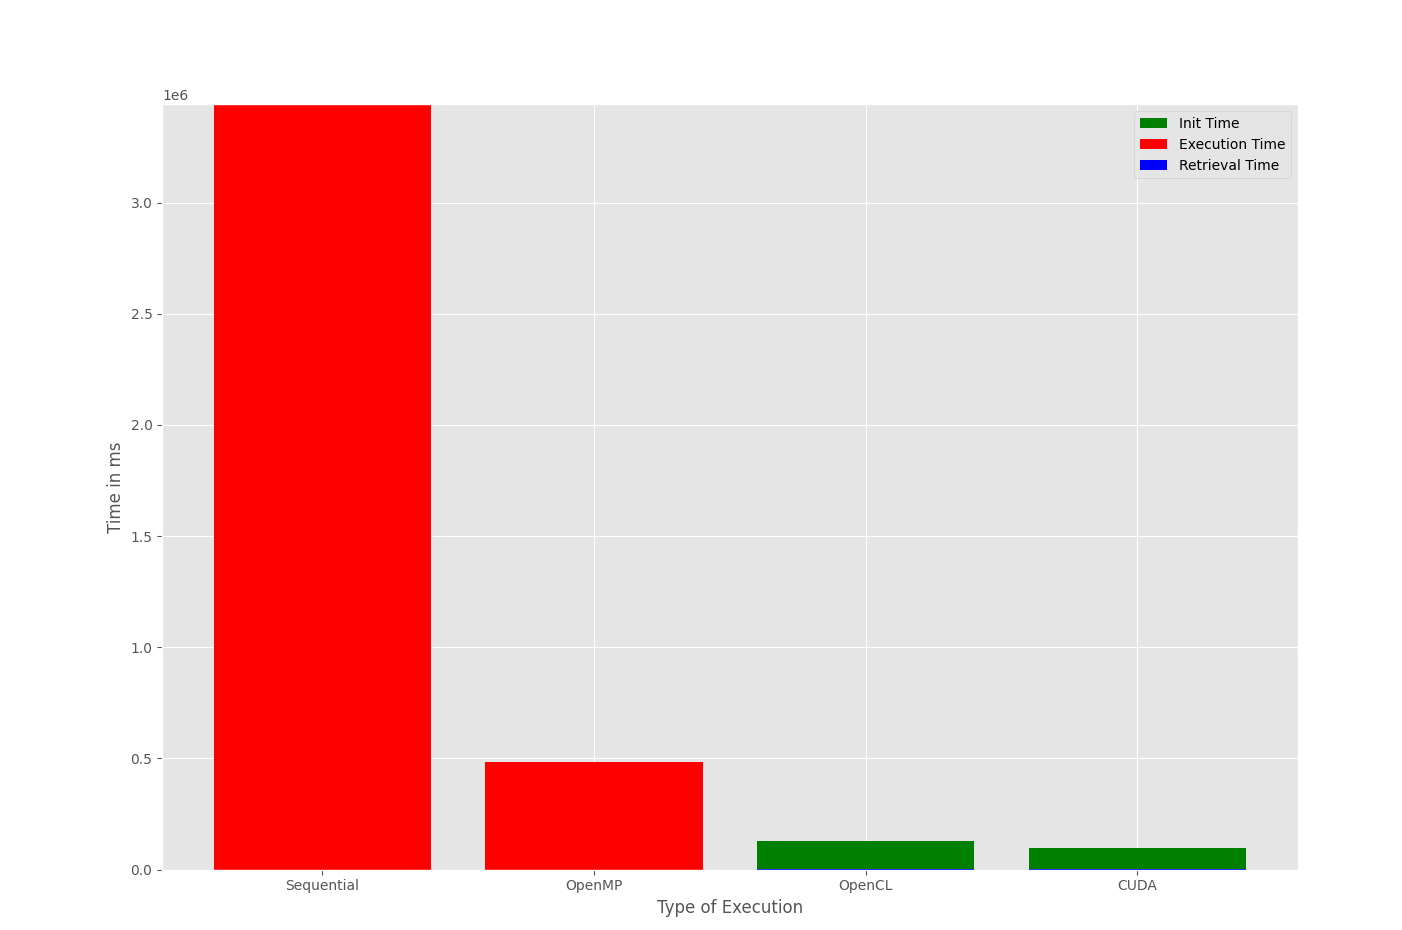
\includegraphics[width=\linewidth]{figures/results.png}
    \caption{ }
	\label{subfig:a}
  \end{subfigure}    
  \begin{subfigure}{0.45\textwidth}
    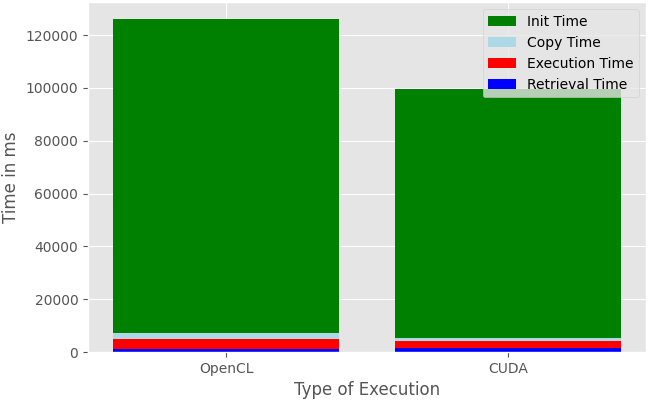
\includegraphics[width=\linewidth]{figures/GPUs_Time.png}
    \caption{ }
	\label{subfig:b}
  \end{subfigure}
    \caption{Initialization, Execution and Data Retrieval Time in Milliseconds of Different Implementations}
    \label{fig:time}
  \end{center}
\end{figure}

Figure \ref{fig:time} illustrates the ratios of time difference well.
The red parts of each bar shows the execution time needed to execute the matrix multiplication.
It can be seen that the CPU execution takes much longer than the executions using the GPU programming models --- even the multi-threaded OpenMP version.
Furthermore, subfigure \ref{subfig:b} contains only both GPU bars, so that the parts of these can be seen easier.
It shows that a lot of time is used to prepare the kernel function compared to the actual execution.


\section{Conclusion and Discussion}
Having a growing attention and amount of data in the field of machine learning, general purpose GPUs will become more and more important for these fields.
It offers huge amounts of parallelizable data which will be processed by these accelerators.
This paper showed that GPUs work much faster than CPUs do --- even when utilizing multi-threading.
However, when programming with GPUs, the overhead of moving data has to be considered.
Furthermore, during the implementation of the matrix multiplication in CUDA and OpenCL, it came clear that CUDA is a better choice when it comes to GPU programming.
The lines of code needed to start a kernel function are less.
This makes the programming less complex.
In OpenCL the programs context has to be defined and the parameters have to be passed one by one to the kernel function.
Therefore, the initialization time in OpenCL is much more complex and takes longer than in CUDA.


% Literaturverzeichnis ------------------------------------------------
\newpage
\bibliographystyle{alphadinLinkLocal}
\bibliography{literatur}

%\iffalse
\end{document}
%\fi
